\documentclass[a4j,12pt]{jarticle}
\usepackage[dvipdfmx]{graphicx}
\usepackage[dvipdfmx]{hyperref}
%
% ---- 本文中でプログラムを掲載する際にキャプションを「リスト1」のようにする設定
%
% http://en.wikibooks.org/wiki/LaTeX/Floats,_Figures_and_Captions#Custom_floats
% 本文中でリストと表現されているところは
%
% \begin{program}..\end{program}を使います。
%
%  \begin{program}\centering
%  \begin{verbatim}
%
%  #define COM1_PORT (0x3f8)
%  #define COM1_LSR (COM1_PORT + 0)
%  #define COM1_RBR (COM1_PORT + 5)
%  unsigned char read_reg_byte(unsigned short port) {
%    unsigned char val;
%    asm volatile("inb %1, %0" : "=a"(val) : "Nd"(port));
%    return val;
%  }
%  \end{verbatim}
%  \caption{I/O マップド I/O での read\_reg\_byte() 関数およびレジスタの宣言}
%  \end{program}
%
% TODO: programをリストに変更する
%
\usepackage{float}
% 例では次のようになっているが...
%\newfloat{program}{thp}{lop}
\newfloat{program}{thp}{lop}
% ------------------------------------------------------------------------------

\title{ハイパーバイザの作り方~ちゃんと理解する仮想化技術~ 第 4 回 I/O 仮想化「割り込み編・その 1 」}
 \author{Takuya ASADA syuu@dokukino.com}
\begin{document}
\maketitle

\section{割り込みの種類}

 前回の記事ではI/O仮想化の機能のうち、I/Oデバ
イスへのアクセスをエミュレーションする方法を中
心に解説してきました。今回は、割り込み仮想化の
話の前提となるx86アーキテクチャにおける割り込
みのしくみを解説します。

 CPUが持つ機能として、割り込みというものがあり
ます。これは、現在CPU上で実行しているプログラム
を停止して、別の処理を実行するための機能です。

 CPUより処理速度の遅い周辺機器へのI/Oを非同
期に行うため、周辺機器からCPUへI/O終了を通知
する機能として実装されました。現在では、より広
い用途で用いられています。

\subsection{外部割り込み、内部割り込み}

 割り込みは、外部割り込みと内部割り込みの2種
類に分けられます。外部割り込みとは、ハードウェ
アからCPUへ「キーボード押された」などのイベント
通知を行うのに用いられます。外部割り込みは、さ
らに{\bf マスク可能な割り込み}と
{\bf ソフトウェアからマスク可能な割り込み(NMI)}
の2種類に分類されます。
マスク可能な割り込みは通常のデバイスからの割り
込みに用いられます。また、NMIはハードウェア障
害の通知など一部特殊な用途に用いられます。

 内部割り込みとは、CPU内部の要因で発生する割
り込みのことです。この内部割り込みは、ソフト
ウェア割り込みと例外に分類されます。ソフトウェ
ア割り込みとは、割り込みを起こす命令(INT命令)
により発生する割り込みです。これはシステムコー
ルの実装に用いられます。例外とは、プログラムを
実行した結果としてゼロ除算/オーバーフロー/無
効な命令の実行/ページフォルトなどが発生したと
きなどに起きる割り込みです。これは、CPUで実行
されるプログラムの制御に用いられます。


\section{ベクタ番号と IDT}

 これらすべての種類の割り込みに0-255のベクタ
番号が割り当てられます。例外は要因別に0-19、
NMIは2が固定的に割り当てられています。ソフト
ウェア割り込みは0-255のすべてのベクタ番号を使
用可能、外部割り込みは16-255を使用可能になって
います。

 割り込みを使用するにはIDT(Interrupt Descriptor
Table)と呼ばれる割り込みハンドラのアドレスを格
納する最大255エントリのテーブル(配列)を作成し、
IDTのアドレスをIDTRレジスタに設定する必要が
あります。割り込み発生時、CPUはIDTRの値から
IDTを参照し、指定された割り込みハンドラを実行
します。

 IDTの各エントリはGate Descriptorと呼ばれる
フォーマットで記述されます。これは単なるメモリ
アドレスではなく、セグメントの設定や実行権限
(Ringの値)、リアルモード・プロテクトモードの設
定などいくつかのパラメータを含みます(図\ref{fig1})。

\begin{figure}\centering
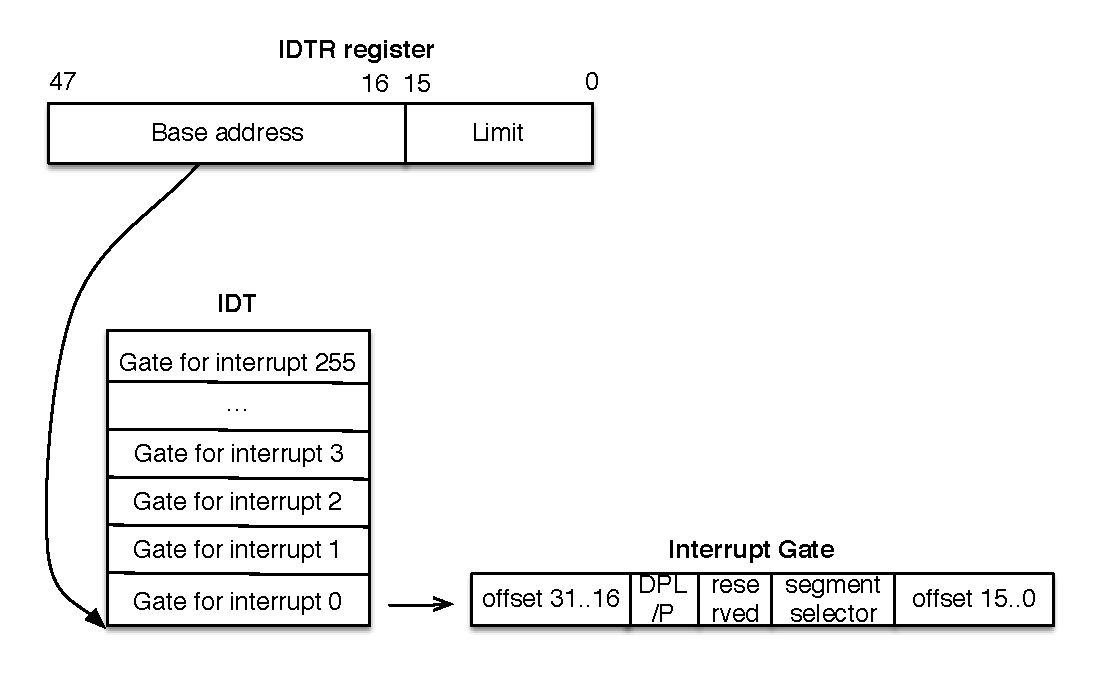
\includegraphics{figures/part4_fig1.eps}
\caption{IDT 、 IDTR 、 Gate descriptor の関係}
\label{fig1}
\end{figure}

 IDTに用いられるGate DescriptorにはTask gate
descriptor/Interrupt gate descriptor/Trap gate
descriptorの3種類があります。しかし、Task gate
descriptorはハードウェアによるマルチタスク機能を
呼び出すためのもので、現代のOSでは使われていま
せん。代わりにInterrupt gate descriptorとTrap gate
descriptorが用いられます。

 この2つの違いは、Interrupt gate descriptorが
EFLAGSレジスタのIFフラグ(割り込みフラグ)を
クリアするのに対して、Trap gate descriptorはIFフ
ラグをクリアしない(割り込みハンドラ内で割り込み
を禁止しない)というものです。

 IDTRレジスタのフォーマットは、IDTの先頭アド
レスとLimit値(テーブルのサイズ)の組み合わせに
なっており、 255未満のテーブルサイズに対応できる
ようになっています。


\section{割り込みのマスク・アンマスク}

 EFLAGSレジスタ(Intel 64ではRFLAGSレジス
タ)のIFフラグをクリアすると割り込みを禁止、IFフ
ラグをセットすると割り込みを有効にすることがで
きます。プログラムからIFフラグをクリア/セット
するには、CLI命令/STI命令を使用します。

 また、前述のとおり、Interrupt Gate Descriptorを
使用して割り込みをハンドルする場合はCPUによっ
て IF フラグがクリアされるため、割り込みは自動
的に禁止されます。このとき、割り込みハンドラを
終了して割り込み前に実行していたプログラムへ制
御を戻すIRET命令を実行すると、割り込み前の
EFLAGSレジスタの値がリストアされ、再び割り込
み可能になります。


\section{外部割り込みと割り込みコントローラ}

 オリジナルのPCアーキテクチャでは、外部割り
込みを制御し、CPUへ伝える役割を受け持つ割り込
みコントローラとしてPIC (i8259)がありました。こ
れは、マザーボード上に存在し、CPUの割り込みラ
インに接続されていました。Pentium以降のx86アー
キテクチャでは、外部割り込みの管理はAPIC
(Advanced Programmable Interrupt Controller)と呼
ばれる新しい割り込みコントローラへ移行され、
PICは互換性のためのみに存在するようになりま
した。APIC は CPU ごとに存在し、CPUに内蔵さ
れているLocal APICと、ICH (Southbridge)に内蔵さ
れているI/O APICから構成されています(図\ref{fig2})。

\begin{figure}\centering
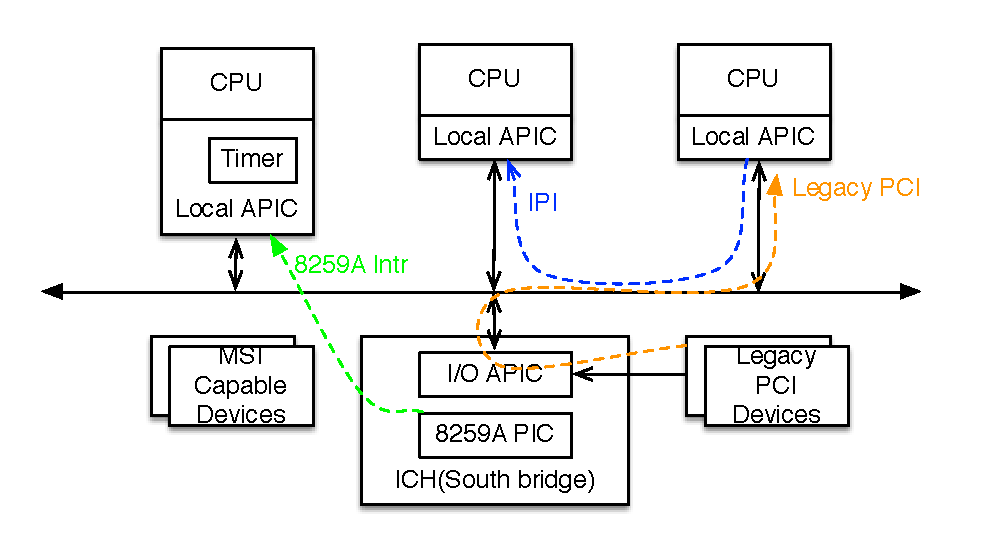
\includegraphics{figures/part4_fig2.eps}
\caption{Local APIC と I/O APIC 、外部デバイスの関係}
\label{fig2}
\end{figure}


 Local APICは、ローカル割り込みのベクタ番号設
定、割り込みベクタ番号通知、EOI (割り込み終了)通
知など、一般的な割り込みコントローラの役割を受
け持ちます。また、タイマー/温度センサ/パ
フォーマンスモニタリングカウンタなどのデバイス、
IPI (プロセッサ間割り込み)の送受信機能を内蔵して
います。

 一方、I/O APICは外部デバイスから割り込みを受
け取り、I/O APIC上の設定に基いて割り込み配信先
のLocal APICを選び割り込みをリダイレクトする
機能を受け持ちます。

 このような構成を取ることによって、SMP環境下
で複数のCPUで外部割り込みを処理できるように
なっています。

 また、あるCPUのLocal APICから別のCPUの
Local APICへIPI ( Inter-Processor Interrupt:プロ
セッサ間割り込み)を送ることもできます。


\section{Local APIC}

 表\ref{table1}に割り込みの処理で利用されるLocal APICの
主なレジスタを示します。

\begin{table}\centering
\begin{tabular}{|p{3cm}|p{3cm}|p{10cm}|} \hline
IRR(Interrupt Request Register) & 割り込み要求レジスタ(Read-only)&
未処理の割り込みを管理するレジスタ。
Local APICに外部割り込みが着信する度にベクタ番号に対応するビットがセットされる。 \\
\hline
ISR(In-Service Register)& インサービスレジスタ(Read-only) &
次に発行される割り込みの候補を管理するレジスタ。
EOIレジスタへ書き込まれるとLocal APICによってIRRから最高優先度のビットがコピーされる。 \\
\hline
EOI(End Of Interrupt)& 割り込み終了レジスタ(Write-only) &
割り込み処理の終了をLocal APICに通知する為のレジスタ。 \\
\hline
TPR(Task Priority Register)&  タスク優先度レジスタ(Read/write) &
外部割り込みに対する実行中タスクの優先度を設定するレジスタ。
TPRに書き込まれた優先度より低い優先度の割り込みはマスクされる。 \\
\hline
PPR(Processor Priority Register)&  プロセッサ優先度レジスタ(Read-only) &
実際の割り込み着信時にマスクを行うか否かの判定に使われるレジスタで、TPRとISRに連動して更新される。 \\
\hline
Local APIC ID Register & LAPIC IDレジスタ(Read/Write) &
システム全体でCPUを一意に特定する為のIDであるLAPIC IDを格納しているレジスタ。
LAPIC IDはI/O APICから外部割り込みを転送する時やIPIを送るときなどに使用される。 \\
\hline
ICR(Interrupt Command Register)& 割り込みコマンドレジスタ(Read/write)& 
IPI(プロセッサ間割り込み)を送信する為のレジスタ。\\
\hline
LDR(Logical Destination Register)&& Logical APIC IDを指定, \\
\hline
DFR(Destination Format Register)&& Logical Destination Modeのモデルを指定(Flat model/Cluster model)\\
\hline
\end{tabular}
\caption{Local APIC の主なレジスタ}
\label{table1}
\end{table}

 割り込み着信時の Local APIC および CPU
の挙動を簡単にまとめると、次のよう流れになります。

\begin{enumerate}
\item Local APICが割り込みを受信したら、IRRに対応す
   るベクタ番号のビットをセットする。CPUが割り
   込みをブロックしている場合はここで処理は終わり
\item IRRにセットされた最高優先度のビットをクリア、
   同じビットをISRにセット、同じ優先度の割り込
   みをCPUへ発行する
\item CPUで割り込みハンドラが実行される
\item CPUで実行された割り込みハンドラがEOIレジス
   タに書き込み、割り込み処理の終了を伝える
\item EOIレジスタへの書き込みを受け取ると、ISRに
   セットされた最高優先度のビットをクリア。まだ
   ISRにビットが残っていたら2から繰り返し
\end{enumerate}

 ただし、タスク優先度/プロセッサ優先度という
機能があり、これによって割り込みに対する実行中
タスクの優先度が制御でき、タスクの優先度が受信
した割り込みより高い場合、その割り込みはマスク
されます。

 TPR ・ PPRレジスタの値は優先度クラス(4-7bit)・
サブ優先度クラス(0-3bit)の2つの値からなり、優先
度クラスだけが割り込みのマスクに使用されます。
先度サブクラスは後述の「Lowest priority Mode」
で使われますが、割り込みのマスクには使用されま
せん。

 PPRの更新はTPRに新しい値が書き込まれたと
きとCPUに割り込みを発行するとき(前述の割り込
み着信時の手順2の段階)に行われます。値は次のよ
うに設定されます。

\begin{figure}\centering
\begin{verbatim}

/* [7:4] は優先度クラス */
/* [3:0] は優先度サブクラス */
if TPR[7:4] >= ISR[7:4]
  PPR = TPR
else
  PPR[7:4] = ISR[7:4]
  PPR[3:0] = 0
\end{verbatim}
\end{figure}

 また、Local APICに割り込みが着信した段階(前
述の割り込み着信時の手順1の段階)で、IRRにセッ
トされた最高優先度のビットとPPRの優先度クラス
(4-7bit)が比較されます。

PPRの優先度クラス(4-7bit)のほうが高かった場合
は割り込みがマスクされます。


\section{I/O APIC}

 I/O APICには外部デバイスからの割り込み線が接
続され、24本の割り込みをサポートしています。各割
り込みの割り込み先はI/O APIC上のRedirection
Tableに設定され、システムバスを通じてCPUの
Local APICへ転送されます。Redirection Tableの各
エントリのフィールドの詳細を表\ref{table2}に示します。

\begin{table}\centering
\begin{tabular}{|p{3cm}|p{3cm}|p{10cm}|} \hline
63:56:00 & Destination & 宛先Local APICの指定 \\ \hline
16 & Mask & 割り込みマスク \\ \hline
15 & Trigger Mode & エッジトリガ/レベルセンシティブ \\ \hline
14 & Remote IRR & レベルセンシティブモードで割り込み送信中/EOI着信済み \\ \hline
13 & Interrupt Pin Polarity & レベルセンシティブモードでhigh/lowのどちらを割り込みリクエストとするか \\ \hline
12 & Delivery Status & 割り込みペンディング中かどうか \\ \hline
11 & Destination Mode & Physical Mode/Logical Mode \\ \hline
10:08 & Delivery Mode & Fixed/Lowest Priorityなど \\ \hline
7:00 & Vector & ベクタ番号 \\ \hline
\end{tabular}
\caption{I/O APIC の Redirection Table Entry}
\label{table2}
\end{table}

 Redirection Table EntryではDestination Modeを
指定する必要があります。Destination Modeに
Physical Destination Modeを指定した場合、 Destination
フィールドにLocal APIC IDを指定することによ
り、宛先CPUを一意に特定します。たとえば、Local
APIC ID: 3のCPUへ割り込みを配信したいときは、
Destinationフィールドに3を指定します。

 Logical Destination Modeを指定した場合、
Destinationフィールドで複数の宛先CPU群をビッ
トマスク指定します
\footnote{これは正確には Logical Flat Model というモードで、他に Flat
     Cluster Model 、 Hierarchical Cluster Model などがあります
     が、通常使われません。説明は割愛します。}
。宛先CPUのIDはLocal
APIC IDではなく、LDRのLogical APIC IDが使用
されます。たとえば、LDRの値が00000001bのCPU
と00000010bのCPUに割り込みを配信したい場合、
Destinationフィールドに00000011bを指定します。

 Logical Destination Modeにより複数のCPUが割
り込み先に指定された時の挙動については、 Delivery
Modeで設定します。Fixed Modeでは、 Destinationに
指定されたすべてのCPUに割り込みます。Lowest
priority Modeでは、 DestinationのうちLocal APICの
TPRが最も小さいCPUへ割り込みます。TPRの値が
最も小さいCPUが複数存在する場合は、ラウンドロ
ビンで割り込みが分散されます
\footnote{Windows ではプロセスごとに TPR の値を制御し、プロセスの
     優先度に多じて割り込み量を変化させています。一方、 Linux
     では TPR の値は変えずに Lowest Priority を用い、複数の CPU
     へ割り込みを公平に分散させています}
。いずれの配信モード
の場合でも、Vectorフィールドで設定されたベク
タ番号でLocal APICへ割り込みがかかります。

 APIC IDのアドレス幅は8bitですので、Logical
Destination Modeでは最大8CPUしかサポートでき
ません。このため、 Nehalem世代よりx2APICと呼ば
れる拡張版APICが導入され、アドレス幅は8bitか
ら32bitへ拡張されました\cite{x2APIC}。

\section{MSI・MSI-X 割り込み}

 I/O APICを経由するPCIデバイスの割り込みは、
各PCIデバイスからの物理的な割り込み線がI/O
APICへ接続され、この割り込み線を通じて割り込
みが送信されていました。

 この構成では割り込みの数とIRQの割り当てが物
理配線に依存するため、限られたIRQを複数のデバ
イスで共有するようなしくみになっていました。ま
た、1つのデバイスで複数の割り込みを持つことはで
きませんでした。この制限を解消するため、物理配
線を用いずPCIバス経由のメッセージとして割り込
みを送るMessage Signalled Interrupt (MSI)・Extended
Message Signalled Interrupt (MSI-X)が導入されてい
ます。PCIではオプション機能として提供されていま
すが、PCI expressでは必須とされています。

 MSIでは各デバイスごとに32個、 MSI-Xでは2048
個の割り込みをサポートします。従来と異なり、デ
バイス間の割り込みは共有されません。MSI ・ MSI-X
の割り込みはIO-APICを経由せず、直接Local
APICへ配送されます(図\ref{fig2}参照)。このとき、宛先
CPUの設定は各PCIデバイスのコンフィギュレー
ションスペースに設定されます。詳細は割愛します
が、コンフィギュレーションスペース内の割り込み
の設定フィールドでは、表2のRedirection Table
Entryに近い内容が割り込みごとに設定できます\cite{interrupt-routing}。

\section{まとめ}

 いかがでしたでしょうか。今回はx86アーキテク
チャにおける割り込みのしくみを解説してきました。
次回は、今回解説した割り込みのしくみをどう仮想
化するかについて解説します。

\section{ライセンス}
Copyright (c) 2014 Takuya ASADA.
全ての原稿データ は クリエイティブ・コモンズ 表示 - 継承 4.0 国際 ライセンスの下に提供されています。

\begin{thebibliography}{4}
  \bibitem{x2APIC} Intel64 Architecture x2APIC Specification \url{http://www.intel.com/content/dam/doc/specification-update/64-architecture-x2apic-specification.pdf}
  \bibitem{interrupt-routing} 最近のPCアーキテクチャにおける割り込みルーティングの仕組み \url{http://d.hatena.ne.jp/syuu1228/20120105/1325757315}
\end{thebibliography}


\end{document}
